%\documentclass[preprints,article,accept,moreauthors,pdftex]{Definitions/mdpi}

\documentclass[computation,article,accept,moreauthors,pdftex]{Definitions/mdpi}

\usepackage[american]{babel}
\usepackage[utf8]{inputenc}
\graphicspath{{./Figures/}}
% If you would like to post an early version of this manuscript as a preprint, you may use preprint as the journal and change 'submit' to 'accept'. The document class line would be, e.g., \documentclass[prepri%nts,article,accept,moreauthors,pdftex]{mdpi}. This is especially recommended for submission to arXiv, where line numbers should be removed before posting. For preprints.org, the editorial staff will make this change immediately prior to posting.

%--------------------
% Class Options:
%--------------------
%----------
% journal
%----------
% Choose between the following MDPI journals:
% acoustics, actuators, addictions, admsci, aerospace, agriculture, agriengineering, agronomy, ai, algorithms, animals, antibiotics, antibodies, antioxidants, applmech, applsci, arts, asc, asi, atmosphere, atoms, axioms, batteries, bdcc, behavsci , beverages, bioengineering, biology, biomedicines, biomimetics, biomolecules, biosensors, brainsci , buildings, cancers, carbon , catalysts, cells, ceramics, challenges, chemengineering, chemistry, chemosensors, children, civileng, cleantechnol, climate, clockssleep, cmd, coatings, colloids, computation, computers, condensedmatter, cosmetics, cryptography, crystals, dairy, data, dentistry, designs , diagnostics, diseases, diversity, drones, econometrics, economies, education, ejbc, ejihpe, electrochem, electronics, endocrines, energies, entropy, environments, epigenomes, est, fermentation, fibers, fire, fishes, fluids, foods, forecasting, forests, fractalfract, futureinternet, futurephys, galaxies, games, gastrointestdisord, gels, genealogy, genes, geohazards, geosciences, geriatrics, hazardousmatters, healthcare, hearts, heritage, highthroughput, horticulturae, humanities, hydrology, ijerph, ijfs, ijgi, ijms, ijtpp, informatics, information, infrastructures, inorganics, insects, instruments, inventions, iot, j, jcdd, jce, jcm, jcp, jcs, jdb, jfb, jfmk, jimaging, jintelligence, jlpea, jmmp, jmse, jne, jnt, jof, joitmc, jpm, jrfm, jsan, land, languages, laws, life, literature, logistics, lubricants, machines, magnetochemistry, make, marinedrugs, materials, mathematics, mca, medicina, medicines, medsci, membranes, metabolites, metals, microarrays, micromachines, microorganisms, minerals, modelling, molbank, molecules, mps, mti, nanomaterials, ncrna, ijns, neurosci, neuroglia, nitrogen, notspecified, nutrients, oceans, ohbm, optics, particles, pathogens, pharmaceuticals, pharmaceutics, pharmacy, philosophies, photonics, physics, plants, plasma, pollutants, polymers, polysaccharides, preprints , proceedings, processes, prosthesis, proteomes, psych, publications, quantumrep, quaternary, qubs, reactions, recycling, religions, remotesensing, reprodmed, reports, resources, risks, robotics, safety, sci, scipharm, sensors, separations, sexes, signals, sinusitis, smartcities, sna, societies, socsci, soilsystems, sports, standards, stats, surfaces, surgeries, sustainability, sustainableworld, symmetry, systems, technologies, telecom, test, tourismhosp, toxics, toxins, transplantology, tropicalmed, universe, urbansci, vaccines, vehicles, vetsci, vibration, viruses, vision, water, wem, wevj

%---------
% article
%---------
% The default type of manuscript is "article", but can be replaced by:
% abstract, addendum, article, benchmark, book, bookreview, briefreport, casereport, changes, comment, commentary, communication, conceptpaper, conferenceproceedings, correction, conferencereport, expressionofconcern, extendedabstract, meetingreport, creative, datadescriptor, discussion, editorial, essay, erratum, hypothesis, interestingimages, letter, meetingreport, newbookreceived, obituary, opinion, projectreport, reply, retraction, review, perspective, protocol, shortnote, supfile, technicalnote, viewpoint
% supfile = supplementary materials

%----------
% submit
%----------
% The class option "submit" will be changed to "accept" by the Editorial Office when the paper is accepted. This will only make changes to the frontpage (e.g., the logo of the journal will get visible), the headings, and the copyright information. Also, line numbering will be removed. Journal info and pagination for accepted papers will also be assigned by the Editorial Office.

%------------------
% moreauthors
%------------------
% If there is only one author the class option oneauthor should be used. Otherwise use the class option moreauthors.

%---------
% pdftex
%---------
% The option pdftex is for use with pdfLaTeX. If eps figures are used, remove the option pdftex and use LaTeX and dvi2pdf.

%=================================================================
\firstpage{1}
\makeatletter
\setcounter{page}{\@firstpage}
\makeatother
\pubvolume{xx}
\issuenum{1}
\articlenumber{5}
\pubyear{2020}
\copyrightyear{2020}
%\externaleditor{Academic Editor: name}
\history{Received: 29 February 2020; Accepted: 24 April 2020; Published: date}
\updates{yes} % If there is an update available, un-comment this line
%%\history{Received: date; Accepted: date; Published: date}

%\%updates{yes} % If there is an update available, un-comment this line

\usepackage{amsmath}

% Line breaks in URLs
\usepackage{url}
\def\UrlBreaks{\do\/\do-}

% Try to avoid widows and orphans
\clubpenalty = 10000
\widowpenalty = 10000
\displaywidowpenalty = 10000

\definecolor{BrickRed}{rgb}{0.8, 0.25, 0.33}
\newcommand{\review}[1]{{\color{BrickRed}#1}}

\Title{Accurate Sampling with Noisy Forces from Approximate Computing}%Attention AE/ME. The following layout issues have not been checked by the English Editing Department and must be carefully verified by the AE/Layout Department: All callout issues, bold usage of callouts, and references to callouts in the text. Correct callout usage in figures. Figure and Table layout issues. Footnote formatting and Glossaries have not been checked. En dash usage for negative values, en dash usage to indicate relationships, en dash usage to indicate bonds (especially in chemistry). The English Editing Department is not responsible for correct italic usage for genes, proteins and technical terminology. This responsibility belongs to the authors. The following are also not checked: spacing between numbers and units of measurement, ratios, en dashes for ranges, date and time formats, punctuation in equation lines, and less than/more than spacing (< >). Finally, capitalization and layout of titles/headings must be properly checked as well as ensuring 'Eq.' and 'Fig.' are properly spelled out, as these are layout issues.

% Author Orchid ID: enter ID or remove command
\newcommand{\orcidauthorA}{0000-0001-5728-9982} % Plessl Add \orcidA{} behind the author's name
\newcommand{\orcidauthorB}{0000-0001-5471-2407} % Kühne Add \orcidB{} behind the author's name
\newcommand{\orcidauthorC}{0000-0002-5708-7632} % Lass Add \orcidC{} behind the author's name

% Authors, for the paper (add full first names)
%\Author{Varadarajan Rengaraj $^{1,\dagger,\ddagger}$\orcidA{}, Firstname Lastname $^{1,\ddagger}$ and Firstname Lastname $^{2,}$*}

\Author{Varadarajan %Please carefully check the accuracy of names and affiliations. Changes will not be possible after proofreading.
 Rengaraj $^{1,2,\dag}$, Michael Lass $^{2,3,\dag}\orcidC{}$, Christian Plessl $^{2,3}$\orcidA{} and Thomas D. Kühne $^{1,4,}$*\orcidB{}}


% Authors, for metadata in PDF
\AuthorNames{Varadarajan Rengaraj, Michael Lass, Christian Plessl and Thomas D. Kühne}

% Affiliations / Addresses (Add [1] after \address if there is only one affiliation.)
\address{%
$^{1}$ \quad Dynamics of Condensed Matter, Department of Chemistry, Paderborn University, Warburger Str. 100, 33098~Paderborn, Germany; rengaraj@campus.uni-paderborn.de\\
$^{2}$ \quad Department of Computer Science, Paderborn University, Warburger Str. 100, 33098 Paderborn, Germany; \hl{michael.lass@uni-paderborn.de} (M.L.); christian.plessl@uni-paderborn.de (C.P.)\\
$^{3}$ \quad Paderborn Center for Parallel Computing, Paderborn University, Warburger Str. 100, 33098 Paderborn, Germany\\
$^{4}$ \quad Center for Sustainable Systems Design, Paderborn University, Warburger Str. 100, 33098 Paderborn, Germany
}

% Contact information of the corresponding author
%\corres{Correspondence: christian.plessl@uni-paderborn.de}
\corres{Correspondence: tdkuehne@mail.upb.de}

% Current address and/or shared authorship
%\firstnote{Current address: Affiliation 3}
\firstnote{These authors contributed equally to this work.}
% The commands \thirdnote{} till \eighthnote{} are available for further notes

\abstract{
In scientific computing, the acceleration of atomistic computer simulations by means of custom hardware is finding ever-growing application.
A major limitation, however, is that the high efficiency in terms of performance and low power consumption entails the massive usage of low precision computing units. Here, based on the approximate computing paradigm, we present an algorithmic method to compensate for numerical inaccuracies due to low accuracy arithmetic operations rigorously, yet still obtaining exact expectation values using a properly modified Langevin-type equation.
}

\keyword{
approximate computing; CP2K; fluctuation-dissipation theorem; FPGA; i-PI; low precision arithmetic
}



%\author[dcm,cs]{Varadarajan Rengaraj}
%\ead{rengaraj@campus.uni-paderborn.de}
%\author[cs,pc2]{Michael Lass\corref{corauthor}}
%\ead{michael.lass@uni-paderborn.de}
%\author[cs,pc2]{Christian Plessl}
%\ead{christian.plessl@uni-paderborn.de}
%\author[dcm,pc2,cssd]{Thomas D. K\"uhne}
%\ead{tdkuehne@mail.upb.de}

%\cortext[corauthor]{Corresponding author}

%\address[dcm]{Dynamics of Condensed Matter, Department of Chemistry, \\ Paderborn University, Warburger Str. 100, 33098 Paderborn, Germany}
%\address[cs]{Department of Computer Science, \\ Paderborn University, Warburger Str. 100, 33098 Paderborn, Germany}
%\address[pc2]{Paderborn Center for Parallel Computing, \\ Paderborn University, Warburger Str. 100, 33098 Paderborn, Germany}
%\address[cssd]{Center for Sustainable Systems Design, \\ Paderborn University, Warburger Str. 100, 33098 Paderborn, Germany}

\begin{document}

%\review{Modified parts are highlighted}

%%%%%%%%%%%%%%%%%%%%%%%%%%%%%%%%%%%%%%%%%%%%%%%%%%%%%%%%%%%%%%%%%%%%%%%%%%%%%%%%%%%%%%%%%%
\section{Introduction}
%%%%%%%%%%%%%%%%%%%%%%%%%%%%%%%%%%%%%%%%%%%%%%%%%%%%%%%%%%%%%%%%%%%%%%%%%%%%%%%%%%%%%%%%%%

Molecular dynamics (MD) is a very powerful and widely used technique to study thermodynamic equilibrium properties, as~well as the real-time dynamics of complex systems made up of interacting atoms~\cite{AlderWainwright1957}. This is done by numerically solving Newton's equations of motion in a time-discretized fashion via computing the nuclear forces of all atoms at every time step~\cite{RahmanMD}. Computing these forces by analytically differentiating the interatomic potential with respect to the nuclear coordinates is computationally rather expensive, which is particularly true for electronic structure-based {ab-initio} MD simulations~\cite{CPMD, CPMD_TDK, PayneRMP, WIRES_TDK}.

For a long time, newly developed microchips have bec\hl{o}me faster and more efficient due to new manufacturing processes and shrinking transistor sizes. However, this development is slowly coming to an end as scaling down the structures of silicon-based chips becomes more and more difficult. The~focus therefore shifts towards making efficient use of the available technology. Hence, besides~algorithmic developments~\cite{MTS, Snir, GSE, Shaw, VerletCell, pSHAKE, John, Prodan}, there have been numerous custom computing efforts in this area to increase the efficiency of MD simulations by means of hardware acceleration, which~we take up~in this~work. Examples of the latter are MD implementations on graphics processing units (GPUs)~\cite{HOOMD, NAMD, OpenMM, HalMD, Lammps, Amber, Gromacs}, field-programmable gate arrays (FPGAs) \cite{HerbordtI, HerbordtII}, and~application-specific integrated~circuits (ASICs)~\cite{AntonI, AntonII}.
While the use of GPUs for scientific applications is relatively widespread~\cite{GPUcomp,Binder,Weigel}, the~use of ASICs~\cite{QCDScience, QCDOC, GrapeScience, Grape} and FPGAs is less common~\cite{JanusI, JanusII, Convey, FDTD, Kenter, Galerkin}, but~has gained attention over the last few years.
In general, to~maximize the computational power for a given silicon area, or~equivalently minimize the power-consumption per arithmetic operation, more and more computing units are replaced with lower precision units. This trend is mostly driven by the market considerations of the gaming and artificial intelligence industries, which are the target customers of hardware accelerators and naturally do not absolutely rely on full computing~accuracy.

In the approach presented in this paper, we {mimic in software how it is possible to} make effective use of low accuracy special-purpose hardware for general-purpose scientific computing by leveraging the approximate computing (AC) paradigm~\cite{KlavikMalossiBekasEtAl2014, PlesslAC}. The~general research goal of AC is to devise and explore ingenious techniques to relax the exactness of a calculation to facilitate the design of more powerful and/or more efficient computer systems. However, in~scientific computing, where the exactness of all computed results is of paramount importance, attenuating accuracy requirements is not an option. Yet, {assuming that the inaccuracies within the nuclear forces due to the usage of low precision arithmetic operations can be approximately considered as white noise}, we will demonstrate that it is nevertheless possible to compensate for such numerical errors rigorously and still obtain exact expectation values, as~obtained by ensemble averages of a properly modified Langevin~equation.

The remainder of the paper is organized as follows. In~Section~\ref{sec:ac}, we revisit the basic principles of AC before introducing our modified Langevin equation in Section~\ref{sec:methodology}. Thereafter, in~Section~\ref{sec:computational}, we~describe the computational details of our computational experiments. Our results are presented and discussed in Section~\ref{sec:results} before concluding the paper in Section~\ref{sec:conclusion}.


%%%%%%%%%%%%%%%%%%%%%%%%%%%%%%%%%%%%%%%%%%%%%%%%%%%%%%%%%%%%%%%%%%%%%%%%%%%%%%%%%%%%%%%%%%
\section{Approximate~Computing}
%%%%%%%%%%%%%%%%%%%%%%%%%%%%%%%%%%%%%%%%%%%%%%%%%%%%%%%%%%%%%%%%%%%%%%%%%%%%%%%%%%%%%%%%%%
\label{sec:ac}

A basic method of approximation and a key requirement for efficient use of processing hardware is the use of adequate data widths in computationally intensive kernels. While in many scientific applications, the use of the double-precision floating-point is most common, this precision is not always required.
For example, iterative methods can exhibit resilience against low precision arithmetic, as has been shown for the computation of inverse matrix roots~\cite{lass17-esl} and for solving systems of linear equations~\cite{KlavikMalossiBekasEtAl2014,Bekas,Dongarra2017,Dongarra2018}.
Mainly driven by the growing popularity of artificial neural networks~\cite{Gupta2015}, we~can observe growing support of low precision data types
in hardware accelerators.
In fact, recent GPUs targeting the data center have started supporting half-precision as well, nearly doubling the peak performance compared to single-precision and quadrupling it compared to double-precision arithmetics~\cite{tesla}. However, due to the low number of exponent bits, half-precision only provides a very limited dynamic range. In~contrast, \texttt{bfloat16} %please check the use of the font; define if appropriate
 provides the same dynamic range as single-precision and~just reduces precision. It is currently supported by Google's Tensor Processing Units (TPU)~\cite{tpu}, and support has been announced for future Intel Xeon processors~\cite{xeon} and Intel AgileX FPGAs. A~list of commonly used data types, together with the corresponding number of bits used to store the exponent and the mantissa, are shown in Table~\ref{tab:float} beside the double-precision {de facto} standard. 

\begin{table}[H]
 \caption{Bitwidth of common floating-point~formats.}
 \centering
 \label{tab:float}
 \begin{tabular}{lrrr}
 \toprule
 \textbf{Type} & \textbf{Sign} & \textbf{Exponent} & \textbf{Mantissa} \\
 \midrule
 IEEE 754 quadruple-precision & 1 & 15 & 112 \\
 IEEE 754 double-precision & 1 & 11 & 52 \\
 IEEE 754 single-precision & 1 & 8 & 23 \\
 IEEE 754 half-precision & 1 & 5 & 10 \\
 Bfloat16%define if appropriate
 (truncated IEEE single-precision) & 1 & 8 & 7\\
 \bottomrule
 \end{tabular}
\end{table}

Yet, programmable hardware such as FPGAs, as~a platform for custom-built accelerator designs~\cite{Strzodka2006, KenterVector, KenterPragma}, can make effective use of all of these, but~also entirely custom number formats.
Developers can specify the number of exponent and mantissa bits and trade-off precision against the amount of memory blocks required to store values and the number of logic elements required to perform arithmetic operations on~them.

In addition to floating-point formats, also fixed-point representations can be used. Here, all~numbers are stored as integers of a fixed size with a
predefined scaling factor. Calculations are thereby performed using integer arithmetic. On~CPUs and GPUs, only certain models can perform integer operations with a peak performance similar to that of floating-point arithmetic, depending on the capabilities of the vector units/stream processors. Nevertheless, FPGAs typically can perform integer operations with performance similar to or even higher than that of the floating-point. Due to the high flexibility of FPGAs with respect to different data formats and the possible use of entirely custom data types, we see them as the main target technology for our work. For~this reason, we consider both floating-point and fixed-point arithmetic in the~following.

%%%%%%%%%%%%%%%%%%%%%%%%%%%%%%%%%%%%%%%%%%%%%%%%%%%%%%%%%%%%%%%%%%%%%%%%%%%%%%%%%%%%%%%%%%
\section{Methodology}
%%%%%%%%%%%%%%%%%%%%%%%%%%%%%%%%%%%%%%%%%%%%%%%%%%%%%%%%%%%%%%%%%%%%%%%%%%%%%%%%%%%%%%%%%%
\label{sec:methodology}
{
The error introduced by low precision floating-point or fixed-point computations can in general be modeled as white noise if unbiased rounding techniques are used in all arithmetic operations. %Such rounding techniques round to the nearest value and use a tie break that does not introduce a systematic bias. 
A~widely employed rounding technique is {round half to even}, which does not introduce a systematic bias and~is used by default in IEEE 754 floating-point arithmetic~\cite{IEEE2019}. In~the following, we assume the usage of such a rounding technique also for fixed-point arithmetic, leading to only an unbiased error within the computed interatomic forces. 
%This has been verified by computing the following series with double-precision, fixed-point arithmetic with three decimal bits and floating-point arithmetic with three mantissa bits. In all cases, \emph{round to nearest, round half to even} has been used as rounding technique, which is the default for IEEE 754 floating-point.
%\begin{eqnarray*}
% R_{1\dots 100,000} &\leftarrow& \text{random values in } [0,1]\\
% S_1 &=& R_1\\
% S_i &=& S_{i-1}\cdot R_i + 0.5\cdot R_i\quad\text{for } i=2\dots 100,000
%\end{eqnarray*}
%Figures \dots show autocorrelation plots for the error $S^{fix} - S^{double}$ and $S^{float} - S^{double}$.
}

To demonstrate the concept of approximate computing, we introduce white noise to the interatomic forces that are computed while running the MD simulation. In~this section, we describe in detail how we introduce the noise to mimic in software the behavior that would be observed when running the MD on the actual FPGA or GPU hardware with reduced numerical precision. We classify the computational errors into two types: fixed-point errors and~floating-point errors. Assuming that $\textbf{F}_{I}$ are the exact and $\textbf{F}_{I}^{N}$ the noisy forces from {an MD simulation} with low precision on an FPGA for instance, fixed-point errors can by modeled by:
\begin{equation}
\textbf{F}_{I}^{N}=
\begin{pmatrix}
\text{F}_{I}^{x}\\
\text{F}_{I}^{y}\\
\text{F}_{I}^{z}\\
\end{pmatrix} +
\begin{pmatrix}
c_{1} \times 10^{-\beta }\\
c_{2} \times 10^{-\beta }\\
c_{3} \times 10^{-\beta }\\
\end{pmatrix}
,
\end{equation}

\noindent whereas floating-point errors are described by:
\begin{equation}
\textbf{F}_{I}^{N} =
\begin{pmatrix}
\text{F}_{I}^{x} \times 10^{-\alpha_1}\\
\text{F}_{I}^{y} \times 10^{-\alpha_2}\\
\text{F}_{I}^{z} \times 10^{-\alpha_3}\\
\end{pmatrix} +
\begin{pmatrix}
c_{1} \times 10^{-(\alpha_1+\beta)}\\
c_{2} \times 10^{-(\alpha_2+\beta)}\\
c_{3} \times 10^{-(\alpha_3+\beta)}\\
\end{pmatrix}
.
\end{equation}

 Therein, $c_1$, $c_2$, and $c_3$ are random values chosen in the range [-0.5, 0.5], whereas $\text{F}_{I}^{x}$, $\text{F}_{I}^{y}$, and $\text{F}_{I}^{x}$ are the individual force components of $\textbf{F}_{I}$, respectively. The~floating-point scaling factor is denoted as $\alpha$ and the magnitude of the applied noise by \(\beta\).

To correct the errors introduced by numerical noise rigorously, we employ a modified Langevin equation. In~particular, we model the force as obtained by a low precision computation on a GPU or FPGA-based accelerator as:
\begin{equation} \label{fFPGA}
\textbf{F}_{I}^{N} = \textbf{F}_{I} + \mathbf{\Xi }_{I}^{N},
\end{equation}

\noindent where $\mathbf{\Xi }_{I}^{N}$ is an additive white noise for which:
\begin{equation} \label{CrossCorr}
 \left \langle \textbf{F}_{I}\left ( 0 \right ) \mathbf{\Xi } _{I}^{N}\left ( t \right )\right \rangle \cong 0
\end{equation}

\noindent holds. Throughout, $\langle \cdots \rangle$ denotes Boltzmann-weighted ensemble averages as obtained by the partition function $Z=\text{Tr} \exp(-E/k_B T)$, where $E$ is the potential energy, $k_B$ the so-called Boltzmann constant, and~$T$ the temperature. Given that $\mathbf{\Xi }_{I}^{N}$ is unbiased, which in our case is true by its very definition, it is nevertheless possible to sample the Boltzmann distribution accurately by means of a Langevin-type equation~\cite{Krajewski,Richters,Karhan}, which in its general form reads as:
\begin{equation} \label{LangevinEq}
M_{I}\ddot{\textbf{R}}_{I}=\textbf{F}_{I}+\mathbf{\Xi }_{I}^{N}-\gamma _{N}M_{I}\dot{\textbf{R}}_{I},
\end{equation}

\noindent where $\dot{\textbf{R}}_{I}$ are the nuclear coordinates (the dot denotes the time derivative), $M_I$ are the nuclear masses, and $\gamma _{N}$ is a damping coefficient,
which is chosen to compensate for \(\mathbf{\Xi }_{I}^{N}\). The~latter, in~order to guarantee an accurate canonical sampling, has to obey
the fluctuation-dissipation theorem:
\begin{equation}
\left \langle \mathbf{\Xi }_{I}^{N}\left ( 0 \right ) \mathbf{\Xi }_{I}^{N}\left ( t \right ) \right \rangle \cong 2 \gamma_{N} M_I k_{B} T \delta \left ( t \right ).
\label{FDT}
\end{equation}

\noindent Substituting Equation~(\ref{fFPGA}) into Equation~(\ref{LangevinEq}) results in the desired modified Langevin equation:
\begin{equation} \label{modLangevin}
M_{I}\ddot{\textbf{R}}_{I} = \textbf{F}_{I}^{N}-\gamma _{N}M_{I}\dot{\textbf{R}}_{I},
\end{equation}

\noindent which will be used throughout the remainder of this paper. This is to say that the noise, as~originating from a low precision computation, can be thought of as the additive white noise {of a damping coefficient} $\gamma_N$, which satisfies the fluctuation-dissipation theorem of Equation~(\ref{FDT}). The~specific value of $\gamma_N$ is determined in such a way so as to generate the correct average temperature, as~measured by the equipartition theorem:
\begin{equation}
\left\langle \frac{1}{2} M_I \dot{\textbf{R}}_{I} \right\rangle = \frac{3}{2} k_B T.
\label{EquiPartTheorem}
\end{equation}


%%%%%%%%%%%%%%%%%%%%%%%%%%%%%%%%%%%%%%%%%%%%%%%%%%%%%%%%%%%%%%%%%%%%%%%%%%%%%%%%%%%%%%%%%%
\section{Computational~Details}
%%%%%%%%%%%%%%%%%%%%%%%%%%%%%%%%%%%%%%%%%%%%%%%%%%%%%%%%%%%%%%%%%%%%%%%%%%%%%%%%%%%%%%%%%%
\label{sec:computational}
To demonstrate our approach, we implemented it in the CP2K suite of programs~\cite{CP2Ka, CP2Kb}. More precisely, we conducted MD simulations of liquid silicon (Si) at 3000~K using the environment-dependent interatomic potential of Bazant~et~al.~\cite{EIP1,EIP2}.
All simulations consisted of 1000~Si atoms in a 3D-periodic cubic box of length 27.155~\AA. Using the algorithm of Ricci and Ciccotti~\cite{Ricci}, Equation~(\ref{LangevinEq}) was integrated with a discretized time step of 1.0~fs with $\gamma_N = 0.001~$fs$^{-1}$.

Whereas the latter settings were used to compute our reference data, in~total, six different cases of fixed-point and floating-point errors were investigated by varying the exponent $\beta$ between zero (huge noise) and three (tiny noise) that is, ranging from $1/1000$ of the physical force up to the same magnitude as the force.
As already alluded to above, the~additive white noise is compensated via Equation~(\ref{modLangevin}) by %varying $\gamma_N$ on-the-fly using a Berendsen-like algorithm until the equipartition theorem of Equation~(\ref{EquiPartTheorem}) is satisfied~\cite{Berendsen,TDKwater,TDKrev}.
continuously adjusting the friction coefficient $\gamma_N$ using the adaptive Langevin technique of Leimkuhler and coworkers so as to satisfy the equipartition theorem of Equation~(\ref{EquiPartTheorem})~\cite{JonesLeimkuhler2011, Mones2015, LeimkuhlerStoltz2019}. In~this method, $\gamma_N$~is reinterpreted as a dynamical variable, defined by a negative feedback loop control law as in the Nos\'e--Hoover scheme~\cite{Nose,Hoover}. The~corresponding dynamical equation for $\gamma_N$ reads as:
\begin{equation}
 \dot{\gamma}_N= (2K-n k_B T)/\mathcal{Q},
\end{equation}

\noindent where $K$ is the kinetic energy, $n$ is the number of degrees of freedom, and $\mathcal{Q}=k_B T \tau^2_{NH}$ is the Nos\'e--Hoover fictitious mass with time constant $\tau_{NH}$. Alternatively, $\gamma_N$ can be estimated by integrating the autocorrelation function of the additive white noise~\cite{RZK}.
In Table~\ref{tab:gamma}, the resulting values of \textit{\(\gamma_N^{fix}\)} for fixed-point and \textit{\(\gamma_N^{float}\)} for floating-point errors are reported as a function of \textit{\(\beta\)}.
\begin{table}[H]
 \caption{Values for \textit{\(\gamma_N^{fix}\)} and \textit{\(\gamma_N^{float}\)} as a function of \textit{\(\beta\)}.}
 \centering
 \label{tab:gamma}
 \begin{tabular}{lrr}
 \toprule
 \boldmath{\textit{\(\beta\)}} & \boldmath{\textit{\(\gamma_N^{fix}\)}} & \boldmath{\textit{\(\gamma_N^{float}\)}} \\
 \midrule
 0 &   & 0.00025 \\
 1 & 0.0004 & 0.000005 \\
 2 & 0.000009 & 0.000005 \\
 3 & 0.0000009 &\\
 \bottomrule
 \end{tabular}
\end{table}
\unskip


%%%%%%%%%%%%%%%%%%%%%%%%%%%%%%%%%%%%%%%%%%%%%%%%%%%%%%%%%%%%%%%%%%%%%%%%%%%%%%%%%%%%%%%%%%
\section{Results and~Discussion}
%%%%%%%%%%%%%%%%%%%%%%%%%%%%%%%%%%%%%%%%%%%%%%%%%%%%%%%%%%%%%%%%%%%%%%%%%%%%%%%%%%%%%%%%%%
\label{sec:results}
As can be directly deduced from Table~\ref{tab:gamma}, the~smaller values of $\gamma_N$ for a given $\beta$ immediately suggested a higher noise resilience when using floating-point as compared to fixed-point~numbers.

In Figures~\ref{Fig1} and \ref{Fig2}, the~Si-Si partial pair-correlation function $g(r)$, which describes how the particle-density varies as a function of distance from a reference particle (atoms, molecules, colloids, etc.), as~computed using an optimal scheme for orthorhombic systems~\cite{KAF}, is shown for different values of $\beta$.
As can be seen, for~both fixed-point and floating-point errors, the~agreement with our reference calculation was nearly perfect up to the highest noise we investigated. As~already anticipated earlier, the~usage of floating-point errors was not only able to tolerate higher noise levels, but~was also more~accurate throughout.

To verify that the sampling was indeed canonical, in~Figure~\ref{Fig3}, the actual kinetic energy distribution as obtained by our simulations using noisy forces is depicted and compared to the analytic Maxwell distribution. It was evident that if sampled long enough, not only the mean value, but~also the distribution tails were in excellent agreement with the exact Maxwellian kinetic energy distribution, which demonstrated that we were indeed performing a canonical~sampling.

\begin{figure}[H]
\begin{center}
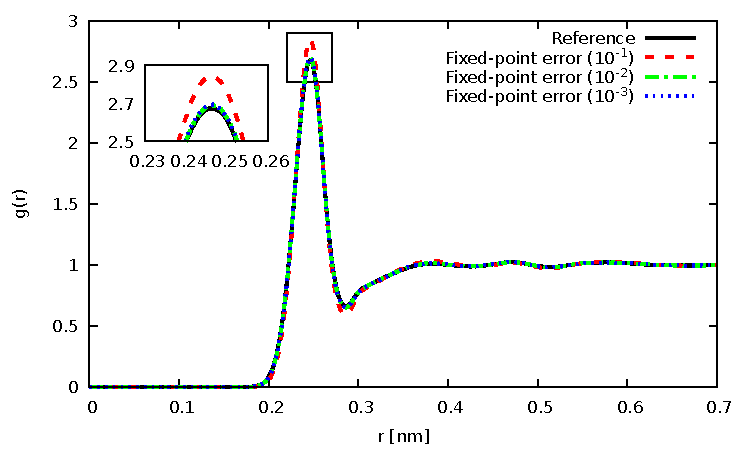
\includegraphics[width=0.8\textwidth]
{Fixed_point_rdf2.pdf}
\end{center}
\caption{\label{Fig1}
Partial pair correlation function for liquid Si at 3000~K with noisy forces introduced by fixed-point errors of magnitude $10^{-3}$ (blue), $10^{-2}$ (green), and $10^{-1}$ (red). For~comparison, the~results, as~obtained by our reference calculations without noise, are shown in black.
} \end{figure}%in the figures throughout, use () not [] around units
\begin{figure}[H]
\begin{center}
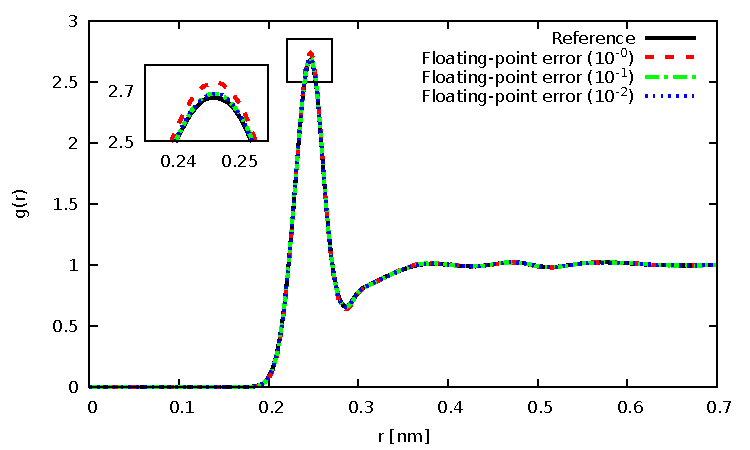
\includegraphics[width=0.8\textwidth]
{Floating_point_rdf2.pdf}
\end{center}
\caption{\label{Fig2}
Partial pair correlation function for liquid Si at 3000~K with noisy forces introduced by floating-point errors of magnitude $10^{-2}$ (blue), $10^{-1}$ (green), and $10^{-0}$ (red). For~comparison, the~results, as~obtained by our reference calculations without noise, are shown in black.
} \end{figure}


\begin{figure}[H]
\begin{center}
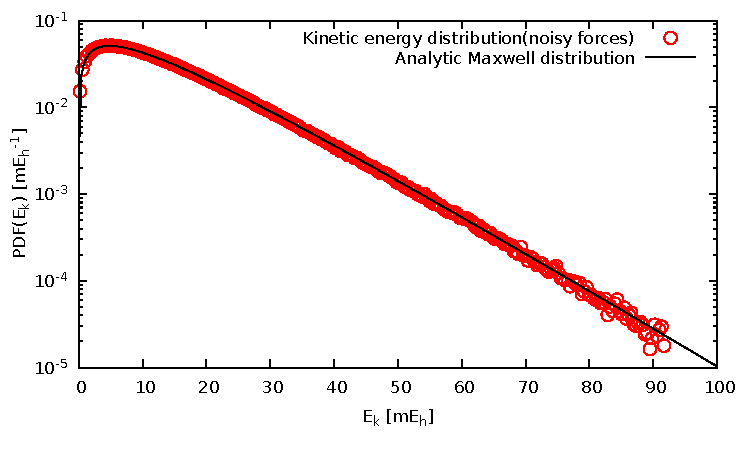
\includegraphics[width=0.8\textwidth]
{maxwelldistribution_new.pdf}
\end{center}
\caption{\label{Fig3}
Kinetic energy distribution of liquid Si at 3000~K, as~obtained by our simulations using noisy forces (circles). For~comparison, the analytic Maxwell distribution is also shown (line).
} \end{figure}
To further assess the accuracy of the present method, we expanded the autocorrelation of the noisy forces, i.e.,

\begin{subequations}
\begin{eqnarray}
 && \left \langle \textbf{F}_{I}^{N}\left ( 0 \right )\textbf{F}_{I}^{N}\left ( t \right )\right \rangle \\
 &=& \left \langle \left ( \textbf{F}_{I}\left ( 0 \right ) + \mathbf{\Xi } _{I}^{N} \left(0 \right )\right) \left( \textbf{F}_{I}\left ( t \right )+\mathbf{\Xi } _{I}^{N}\left ( t \right )\right) \right \rangle \\
 &=& \left \langle \textbf{F}_{I}\left ( 0 \right ) \textbf{F}_{I}\left ( t \right )\right \rangle + \left \langle \textbf{F}_{I}\left ( 0 \right ) \mathbf{\Xi } _{I}^{N}\left(t \right )\right \rangle \label{AutoCorr} \\
 &+& \left \langle \textbf{F}_{I}\left ( t \right ) \mathbf{\Xi } _{I}^{N}\left(0 \right )\right \rangle + \left \langle \mathbf{\Xi } _{I}^{N}\left(0 \right ) \mathbf{\Xi } _{I}^{N}\left(t \right )\right \rangle. \nonumber
\end{eqnarray}
\end{subequations}

Since the cross-correlation terms between the exact force and the additive white noise were vanishing due to Equation~(\ref{CrossCorr}), comparing the autocorrelation of the noisy forces $\langle \textbf{F}_{I}^{N}(0)\textbf{F}_{I}^{N}(t)\rangle$ with the autocorrelation of the exact forces $\langle \textbf{F}_{I}(0) \textbf{F}_{I}(t)\rangle$ permitted assessing the localization of the last term of Equation~(\ref{AutoCorr}).
The fact that $\langle \textbf{F}_{I}^{N}(0)\textbf{F}_{I}^{N}(t)\rangle$ was essentially identical to $\langle \textbf{F}_{I}(0) \textbf{F}_{I}(t)\rangle$, as~can be seen in Figure~\ref{Fig4}, implied that $\langle \mathbf{\Xi } _{I}^{N}(0) \mathbf{\Xi } _{I}^{N}(t)\rangle$ was very close to a $\delta$-function as required by the fluctuation-dissipation theorem in order to ensure an accurate canonical sampling of the Boltzmann distribution. In~other words, from~this, it followed that our initial assumption underlying Equation~(\ref{modLangevin}), to~model the noise due to a low precision calculation as an additive white noise channel, was~justified.
\begin{figure}[H]
\begin{center}
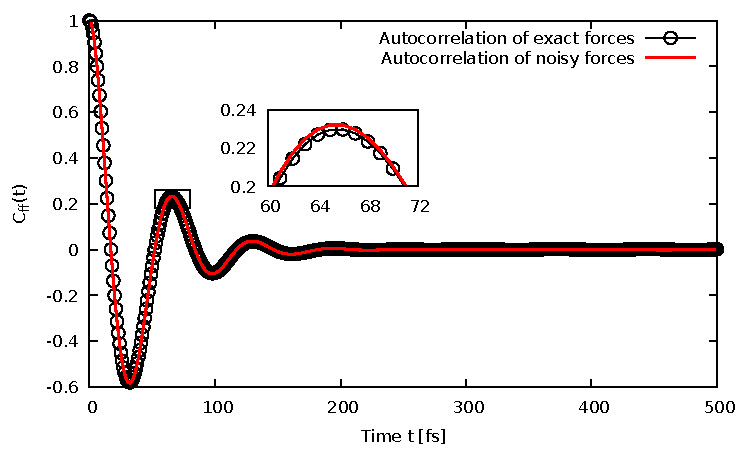
\includegraphics[width=0.8\textwidth]
{AutocorrelationPlot_n.pdf}
\end{center}
\caption{\label{Fig4}
The autocorrelation of the noisy forces \(
\left \langle \textbf{F}_{I}^{N}\left ( 0 \right ) \textbf{F}_{I}^{N}\left ( t \right )\right \rangle \)(line), which are compared to the autocorrelation of the exact forces \( \left \langle \textbf{F}_{I}\left ( 0 \right ) \textbf{F}_{I}\left ( t \right )\right \rangle \)(circles).
} \end{figure}
\unskip

%%%%%%%%%%%%%%%%%%%%%%%%%%%%%%%%%%%%%%%%%%%%%%%%%%%%%%%%%%%%%%%%%%%%%%%%%%%%%%%%%%%%%%%%%%
\section{Conclusions}
%%%%%%%%%%%%%%%%%%%%%%%%%%%%%%%%%%%%%%%%%%%%%%%%%%%%%%%%%%%%%%%%%%%%%%%%%%%%%%%%%%%%%%%%%%
\label{sec:conclusion}
We conclude by noting that the presented method was recently implemented in the universal force engine i-PI~\cite{iPi}, which can be generally applied to all sorts of forces affected by stochastic noise such as those computed by GPUs or other hardware accelerators~\cite{HOOMD, NAMD, OpenMM, HalMD, Lammps, Amber, Gromacs}, and~potentially even quantum computing devices~\cite{Steane, Knill, Blatt, Chow}. The~possibility to apply similar ideas to N-body simulations~\cite{White, Makino} and to combine them with further algorithmic approximations~\cite{LassAC} is to be underlined and will be presented~elsewhere.

%%%%%%%%%%%%%%%%%%%%%%%%%%%%%%%%%%%%%%%%%%
\vspace{6pt} 
%%%%%%%%%%%%%%%%%%%%%%%%%%%%%%%%%%%%%%%%%%
\authorcontributions{\hl{
%For research articles with several authors, a short paragraph specifying their individual contributions must be provided.
V.R. wrote the code and conducted the calculations, 
V.R. and M.L. analyzed the data, M.L., C.P. and 
T.D.K. interpreted the results, M.L., V.R. and T.D.K. 
wrote the paper, C.P. and T.D.K. conceived the study 
and directed the project.}}
%%%%%%%%%%%%%%%%%%%%%%%%%%%%%%%%%%%%%%%%%%%%%%%%%%%%%%%%%%%%%%%%%%%%%%%%%%%%%%%%%%%%%%%%%%

\funding{
The authors would like to thank the Paderborn Center for Parallel Computing (PC$^2$) for computing time on \textsc{OCuLUS} %please check the font; define if appropriate
 and FPGA-based supercomputer \textsc{Noctua}. Funding from Paderborn University's research award for ``Green IT'' is kindly acknowledged. This project has received funding from the European Research Council (ERC) under the European Union's Horizon 2020 research and innovation program (Grant Agreement No.~716142) \hl{and from the German Research Foundation (DFG) under the project PerficienCC (grant agreement No PL 595/2-1)}.}

%%%%%%%%%%%%%%%%%%%%%%%%%%%%%%%%%%%%%%%%%%
\conflictsofinterest{\hl{
%Declare conflicts of interest or state ``The authors declare no conflict of interest.'' 
The authors declare no conflict of interest.
}}

\reftitle{References}
\begin{thebibliography}{999}
%\providecommand{\natexlab}[1]{#1}

\bibitem[Alder and Wainwright(1957)]{AlderWainwright1957}
Alder, B.J.; Wainwright, T.E.
\newblock Phase Transition for a Hard Sphere System.
\newblock {\em J. Chem. Phys.} {\bf 1957}, {\em 27},~1208--1209, doi:10.1063/1.1743957.

\bibitem[Rahman(1964)]{RahmanMD}
Rahman, A.
\newblock Correlations in the Motion of Atoms in Liquid Argon.
\newblock {\em Phys. Rev.} {\bf 1964}, {\em 136},~A405--A411, doi:10.1103/PhysRev.136.A405.

\bibitem[Car and Parrinello(1985)]{CPMD}
Car, R.; Parrinello, M.
\newblock Unified approach for molecular dynamics and density-functional
 theory.
\newblock {\em Phys.~Rev.~Lett.} {\bf 1985}, {\em 55},~2471--2474, doi:10.1103/PhysRevLett.55.2471.

\bibitem[K\"uhne \em{et~al.}(2007)K\"uhne, Krack, Mohamed, and
 Parrinello]{CPMD_TDK}
K\"uhne, T.D.; Krack, M.; Mohamed, F.R.; Parrinello, M.
\newblock Efficient and accurate Car-Parrinello-like approach to
 Born-Oppenheimer molecular dynamics.
\newblock {\em Phys. Rev. Lett.} {\bf 2007}, {\em 98},~066401, doi:10.1103/PhysRevLett.98.066401.

\bibitem[Payne \em{et~al.}(1992)Payne, Teter, Allan, Arias, and
 Joannopoulos]{PayneRMP}
Payne, M.C.; Teter, M.P.; Allan, D.C.; Arias, T.A.; Joannopoulos, J.D.
\newblock Iterative minimization techniques for ab~initio total-energy
 calculations: Molecular dynamics and conjugate gradients.
\newblock {\em Rev. Mod. Phys.} {\bf 1992}, {\em 64},~1045--1097, doi:10.1103/RevModPhys.64.1045.

\bibitem[K\"uhne(2014)]{WIRES_TDK}
K\"uhne, T.D.
\newblock Second generation Car–Parrinello molecular dynamics.
\newblock {\em WIREs Comput. Mol. Sci.} {\bf 2014}, {\em 4},~391--406, doi:10.1002/wcms.1176.

\bibitem[Tuckerman \em{et~al.}(1992)Tuckerman, Berne, and Martyna]{MTS}
Tuckerman, M.E.; Berne, B.J.; Martyna, G.J.
\newblock Reversible multiple time scale molecular dynamics.
\newblock {\em J.~Chem.~Phys.} {\bf 1992}, {\em 97},~1990--2001, doi:10.1063/1.463137.

\bibitem[Snir(2004)]{Snir}
Snir, M.
\newblock A note on N-body computations with cutoffs.
\newblock {\em Theor. Comput. Syst.} {\bf 2004}, {\em 37},~295--318, doi:10.1007/s00224-003-1071-0.

\bibitem[Shan \em{et~al.}(2005)Shan, Klepeis, Eastwood, Dror, and Shaw]{GSE}
Shan, Y.; Klepeis, J.L.; Eastwood, M.P.; Dror, R.O.; Shaw, D.E.
\newblock Gaussian split Ewald: A fast Ewald mesh method for molecular
 simulation.
\newblock {\em J. Chem. Phys.} {\bf 2005}, {\em 122},~054101, doi:10.1063/1.1839571.

\bibitem[Shaw(2005)]{Shaw}
Shaw, D.E.
\newblock A fast, scalable method for the parallel evaluation of
 distance-limited pairwise particle interactions.
\newblock {\em J. Comput. Chem.} {\bf 2005}, {\em 26},~1318--1328, doi:10.1002/jcc.20267.

\bibitem[Gonnet(2012)]{VerletCell}
Gonnet, P.
\newblock Pairwise Verlet Lists: Combining Cell Lists and Verlet Lists to
 Improve Memory Locality and Parallelism.
\newblock {\em J. Comp. Chem.} {\bf 2012}, {\em 33},~76--81, doi:10.1002/jcc.21945.

\bibitem[Gonnet(2007)]{pSHAKE}
Gonnet, P.
\newblock A quadratically convergent SHAKE in O(n(2)).
\newblock {\em J. Comp. Phys.} {\bf 2007}, {\em 220},~740--750, doi:10.1016/j.jcp.2006.05.032.

\bibitem[John \em{et~al.}(2016)John, Spura, Habershon, and K\"uhne]{John}
John, C.; Spura, T.; Habershon, S.; K\"uhne, T.D.
\newblock Quantum ring-polymer contraction method: Including nuclear quantum
 effects at no additional computational cost in comparison to ab~initio
 molecular dynamics.
\newblock {\em Phys. Rev. E} {\bf 2016}, {\em 93},~043305, doi:10.1103/PhysRevE.93.043305.

\bibitem[K\"uhne and Prodan(2018)]{Prodan}
K\"uhne, T.D.; Prodan, E.
\newblock Disordered Crystals from First Principles I: Quantifying the
 Configuration Space.
\newblock {\em Ann. Phys.} {\bf 2018}, {\em 391},~120--149, doi:10.1016/j.aop.2018.01.016.

\bibitem[Anderson \em{et~al.}(2008)Anderson, Lorenz, and Travesset]{HOOMD}
Anderson, J.A.; Lorenz, C.D.; Travesset, A.
\newblock General purpose molecular dynamics simulations fully implemented on
 graphics processing units.
\newblock {\em J. Comp. Phys.} {\bf 2008}, {\em 227},~5342--5359, doi:10.1016/j.jcp.2008.01.047.

\bibitem[Stone \em{et~al.}(2010)Stone, Hardy, Ufimtsev, and Schulten]{NAMD}
Stone, J.E.; Hardy, D.J.; Ufimtsev, I.S.; Schulten, K.
\newblock GPU-accelerated molecular modeling coming of age.
\newblock {\em J.~Mol. Graph. Modell.} {\bf 2010}, {\em 29},~116--125, doi:10.1016/j.jmgm.2010.06.010.

\bibitem[Eastman and Pande(2010)]{OpenMM}
Eastman, P.; Pande, V.S.
\newblock OpenMM: A Hardware-Independent Framework for Molecular Simulations.
\newblock {\em Comput. Sci. Eng.} {\bf 2010}, {\em 12},~34--39, doi:10.1109/MCSE.2010.27.

\bibitem[Colberg and H\"ofling(2011)]{HalMD}
Colberg, P.H.; H\"ofling, F.
\newblock Highly accelerated simulations of glassy dynamics using GPUs: Caveats
 on limited floating-point precision.
\newblock {\em Comp. Phys. Commun.} {\bf 2011}, {\em 182},~1120--1129, doi:10.1016/j.cpc.2011.01.009.

\bibitem[Brown \em{et~al.}(2012)Brown, Kohlmeyer, Plimpton, and
 Tharrington]{Lammps}
Brown, W.M.; Kohlmeyer, A.; Plimpton, S.J.; Tharrington, A.N.
\newblock Implementing molecular dynamics on hybrid high performance computers
 – Particle–particle particle-mesh.
\newblock {\em Comp. Phys. Commun.} {\bf 2012}, {\em 183},~449--459, doi:10.1016/j.cpc.2011.10.012.

\bibitem[{Le Grand} \em{et~al.}(2013){Le Grand}, G\"otz, and Walker]{Amber}
{Le Grand}, S.; G\"otz, A.W.; Walker, R.C.
\newblock SPFP: Speed without compromise---A mixed precision model for GPU
 accelerated molecular dynamics simulations.
\newblock {\em Comp. Phys. Commun.} {\bf 2013}, {\em 184},~374--380, doi:10.1016/j.cpc.2012.09.022.

\bibitem[Abraham \em{et~al.}(2015)Abraham, Murtola, Schulz, Pall, Smith, Hess,
 and Lindahl]{Gromacs}
Abraham, A.J.; Murtola, T.; Schulz, R.; Pall, S.; Smith, J.C.; Hess, B.;
 Lindahl, E.
\newblock GROMACS: High~performance molecular simulations through multi-level
 parallelism from laptops to supercomputers.
\newblock {\em SoftwareX} {\bf 2015}, {\em 1--2},~19--25, doi:10.1016/j.softx.2015.06.001.

\bibitem[Herbordt \em{et~al.}(2008{\natexlab{a}})Herbordt, Gu, VanCourt, Model,
 Sukhwani, and Chiu]{HerbordtI}
Herbordt, M.C.; Gu, Y.; VanCourt, T.; Model, J.; Sukhwani, B.; Chiu, M.
\newblock Computing Models for FPGA-Based Accelerators.
\newblock {\em Comput. Sci. Eng.} {\bf 2008}, {\em 10},~35--45, doi:10.1109/MCSE.2008.143.

\bibitem[Herbordt \em{et~al.}(2008{\natexlab{b}})Herbordt, Gu, VanCourt, Model,
 Sukhwani, and Chiu]{HerbordtII}
Herbordt, M.C.; Gu, Y.; VanCourt, T.; Model, J.; Sukhwani, B.; Chiu, M.
\newblock Explicit design of FPGA-based coprocessors for short-range force
 computations in molecular dynamics simulations.
\newblock {\em Parallel Comput.} {\bf 2008}, {\em 34},~261--277, doi:10.1016/j.parco.2008.01.007.

\bibitem[Shaw \em{et~al.}(2007)Shaw, Deneroff, Dror, Kuskin, Larson, Salmon,
 Young, Batson, Bowers, Chao, Eastwood, Gagliardo, Grossman, Ho, Ierardi,
 Kolossv\'{a}ry, Klepeis, Layman, McLeavey, Moraes, Mueller, Priest, Shan,
 Spengler, Theobald, Towles, and Wang]{AntonI}
Shaw, D.E.; Deneroff, M.M.; Dror, R.O.; Kuskin, J.S.; Larson, R.H.; Salmon,
 J.K.; Young, C.; Batson, B.; Bowers,~K.J.; Chao, J.C.; et al.
\newblock Anton, a Special-purpose Machine for Molecular Dynamics Simulation.
\newblock In~Proceedings~of the 34th Annual International Symposium on Computer
 Architecture, San Diego, CA, USA, 9--13 June 2007; ACM: New York, NY, USA, 2007; pp. 1--12, doi:10.1145/1250662.1250664.

\bibitem[Shaw \em{et~al.}(2014)Shaw, Grossman, Bank, Batson, Butts, Chao,
 Deneroff, Dror, Even, Fenton, Forte, Gagliardo, Gill, Greskamp, Ho, Ierardi,
 Iserovich, Kuskin, Larson, Layman, Lee, Lerer, Li, Killebrew, Mackenzie, Mok,
 Moraes, Mueller, Nociolo, Peticolas, Quan, Ramot, Salmon, Scarpazza,
 Ben~Schafer, Siddique, Snyder, Spengler, Tang, Theobald, Toma, Towles,
 Vitale, Wang, and Young]{AntonII}
Shaw, D.E.; Grossman, J.P.; Bank, J.A.; Batson, B.; Butts, J.A.; Chao, J.C.;
 Deneroff, M.M.; Dror, R.O.; Even, A.; Fenton, C.H.; et al.
\newblock Anton 2: Raising the Bar for Performance and Programmability in a
 Special-purpose Molecular Dynamics Supercomputer.
\newblock In~Proceedings~of the International Conference for High Performance
 Computing, Networking, Storage and Analysis, New Orleans, LA, USA, 16--21 November 2014; IEEE Press: Piscataway, NJ, USA,
 2014; pp. 41--53, doi:10.1109/SC.2014.9.

\bibitem[{Owens} \em{et~al.}(2008){Owens}, {Houston}, {Luebke}, {Green},
 {Stone}, and {Phillips}]{GPUcomp}
{Owens}, J.D.; {Houston}, M.; {Luebke}, D.; {Green}, S.; {Stone}, J.E.;
 {Phillips}, J.C.
\newblock GPU Computing.
\newblock {\em Proc. IEEE} {\bf 2008}, {\em 96},~879--899, doi:10.1109/JPROC.2008.917757.

\bibitem[Preis \em{et~al.}(2009)Preis, Virnau, Paul, and Schneider]{Binder}
Preis, T.; Virnau, P.; Paul, W.; Schneider, J.J.
\newblock GPU accelerated Monte Carlo simulation of the 2D and 3D Ising model.
\newblock {\em J. Comp. Phys.} {\bf 2009}, {\em 228},~4468--4477, doi:10.1016/j.jcp.2009.03.018.

\bibitem[Weigel(2012)]{Weigel}
Weigel, M.
\newblock Performance potential for simulating spin models on GPU.
\newblock {\em J. Comp. Phys.} {\bf 2012}, {\em 231},~3064--3082, doi:10.1016/j.jcp.2011.12.008.

\bibitem[Brown and Christ(1988)]{QCDScience}
Brown, F.R.; Christ, N.H.
\newblock Parallel Supercomputers for Lattice Gauge Theory.
\newblock {\em Science} {\bf 1988}, {\em 239},~1393--1400, doi:10.1126/science.239.4846.1393.

\bibitem[{Boyle} \em{et~al.}(2005){Boyle}, {Chen}, {Christ}, {Clark}, {Cohen},
 {Cristian}, {Dong}, {Gara}, {Joo}, {Jung}, {Kim}, {Levkova}, {Liao}, {Liu},
 {Mawhinney}, {Ohta}, {Petrov}, {Wettig}, and {Yamaguchi}]{QCDOC}
{Boyle}, P.A.; {Chen}, D.; {Christ}, N.H.; {Clark}, M.A.; {Cohen}, S.D.;
 {Cristian}, C.; {Dong}, Z.; {Gara}, A.; {Joo}, B.; {Jung}, C.; et al.
\newblock Overview of the QCDSP and QCDOC computers.
\newblock {\em IBM J. Res. Dev.} {\bf 2005}, {\em
 49},~351--365, doi:10.1147/rd.492.0351.

\bibitem[Hut and Makino(1999)]{GrapeScience}
Hut, P.; Makino, J.
\newblock Astrophysics on the GRAPE Family of Special-Purpose Computers.
\newblock {\em Science} {\bf 1999}, {\em 283},~501--505, doi:10.1126/science.283.5401.501.

\bibitem[Fukushige \em{et~al.}(1999)Fukushige, Hut, and Makino]{Grape}
Fukushige, T.; Hut, P.; Makino, J.
\newblock High-performance special-purpose computers in science.
\newblock {\em Comput. Sci. Eng.} {\bf 1999}, {\em 1},~12--13, doi:10.1109/5992.753041.

\bibitem[Belletti \em{et~al.}(2009)Belletti, Cotallo, Cruz, Fernandez,
 Gordillo-Guerrero, Guidetti, Maiorano, Mantovani, Marinari, Martin-Mayor,
 Munoz-Sudupe, Navarro, Parisi, Perez-Gaviro, Rossi, Ruiz-Lorenzo, Schifano,
 Sciretti, Tarancon, and Tripiccione]{JanusI}
Belletti, F.; Cotallo, M.; Cruz, A.; Fernandez, L.A.; Gordillo-Guerrero, A.;
 Guidetti, M.; Maiorano, A.; Mantovani, F.; Marinari, E.; Martin-Mayor, V.;
 et al.
\newblock Janus: An FPGA-Based System for High-Performance Scientific
 Computing.
\newblock {\em Comput. Sci. Eng.} {\bf 2009}, {\em 11},~48, doi:10.1109/MCSE.2009.11.

\bibitem[Baity-Jesi \em{et~al.}(2014)Baity-Jesi, R.A.~Banos, Cruz, Fernandez,
 Gil-Narvion, Gordillo-Guerrero, Iniguez, Maiorano, Mantovani, Marinari,
 Martin-Mayor, Monforte-Garcia, Munoz-Sudupe, Navarro, Parisi, Perez-Gaviro,
 Pivanti, Ricci-Tersenghi, Ruiz-Lorenzo, Schifano, Seoane, Tarancon,
 Tripiccione, and Yllanes]{JanusII}
Baity-Jesi, M.; R.A.~Banos, R.A.; Cruz, A.; Fernandez, L.A.; Gil-Narvion, J.M.;
 Gordillo-Guerrero, A.; Iniguez,~D.; Maiorano, A.; Mantovani, F.; Marinari,
 E.; et al.
\newblock Janus II: A new generation application-driven computer for
 spin-system simulations.
\newblock {\em Comp. Phys. Commun.} {\bf 2014}, {\em 185},~550--559, doi:10.1016/j.cpc.2013.10.019.

\bibitem[Meyer \em{et~al.}(2012)Meyer, Schumacher, Plessl, and
 Forstner]{Convey}
Meyer, B.; Schumacher, J.; Plessl, C.; Forstner, J.
\newblock Convey vector personalities---FPGA acceleration with an openmp-like
 programming effort?
\newblock In Proceedings of the 22nd International Conference on Field Programmable Logic and Applications (FPL), Oslo, Norway, 29--31 August 2012;
 pp. 189--196, doi:10.1109/FPL.2012.6339259.

\bibitem[Giefers \em{et~al.}(2014)Giefers, Plessl, and F\"{o}rstner]{FDTD}
Giefers, H.; Plessl, C.; F\"{o}rstner, J.
\newblock Accelerating Finite Difference Time Domain Simulations with
 Reconfigurable Dataflow Computers.
\newblock {\em SIGARCH Comput. Archit. News} {\bf 2014}, {\em 41},~65--70, doi:10.1145/2641361.2641372.

\bibitem[Kenter \em{et~al.}(2017)Kenter, F\"orstner, and Plessl]{Kenter}
Kenter, T.; F\"orstner, J.; Plessl, C.
\newblock Flexible FPGA design for FDTD using OpenCL.
\newblock In Proceedings of the 2017 27th International Conference on Field Programmable Logic and Applications (FPL), Ghent, Belgium, 4--8~September~2017; , doi:10.23919/FPL.2017.8056844.

\bibitem[Kenter \em{et~al.}(2018)Kenter, Mahale, Alhaddad, Grynko, Schmitt,
 Afzal, Hannig, F\"orstner, and Plessl]{Galerkin}
Kenter, T.; Mahale, G.; Alhaddad, S.; Grynko, Y.; Schmitt, C.; Afzal, A.;
 Hannig, F.; F\"orstner, J.; Plessl, C.
\newblock OpenCL-based FPGA Design to Accelerate the Nodal Discontinuous
 Galerkin Method for Unstructured Meshes.
\newblock In Proceedings of the 2018 IEEE 26th Annual International Symposium on Field-Programmable Custom Computing Machines (FCCM), Boulder, CO, USA, 29 April--1 May 2018; Volume~1, pp. 189--196, doi:10.1109/FCCM.2018.00037.

\bibitem[Klav{\'\i}k \em{et~al.}(2014)Klav{\'\i}k, Malossi, Bekas, and
 Curioni]{KlavikMalossiBekasEtAl2014}
Klav{\'\i}k, P.; Malossi, A.C.I.; Bekas, C.; Curioni, A.
\newblock {Changing Computing Paradigms Towards Power Efficiency}.
\newblock {\em Philos. Trans. R. Soc. {A}: Math. Phys. Eng. Sci.} {\bf 2014}, {\em 372}, doi:10.1098/rsta.2013.0278.

\bibitem[Plessl \em{et~al.}(2015)Plessl, Platzner, and Schreier]{PlesslAC}
Plessl, C.; Platzner, M.; Schreier, P.J.
\newblock Approximate Computing.
\newblock {\em Inform. Spektrum} {\bf 2015}, {\em 38},~396--399, doi:10.1007/s00287-015-0911-z.

\bibitem[Lass \em{et~al.}(2018)Lass, K\"uhne, and Plessl]{lass17-esl}
Lass, M.; K\"uhne, T.D.; Plessl, C.
\newblock Using Approximate Computing for the Calculation of Inverse Matrix
 p-th Roots.
\newblock {\em IEEE Embed. Syst. Lett.} {\bf 2018}, {\em 10},~33--36.

\bibitem[Angerer \em{et~al.}(2016)Angerer, Polig, Zegarac, Giefers, Hagleitner,
 Bekas, and Curioni]{Bekas}
Angerer, C.M.; Polig, R.; Zegarac, D.; Giefers, H.; Hagleitner, C.; Bekas, C.;
 Curioni, A.
\newblock A fast, hybrid, power-efficient high-precision solver for large
 linear systems based on low precision hardware. {\bf 2016}.
\newblock {\em 12},~72--82, doi:10.1016/j.suscom.2015.10.001.

\bibitem[Haidar \em{et~al.}(2017)Haidar, Wu, Tomov, and Dongarra]{Dongarra2017}
Haidar, A.; Wu, P.; Tomov, S.; Dongarra, J.
\newblock Investigating half precision arithmetic to accelerate dense linear
 system solvers.
\newblock In Proceedings of the 8th Workshop on Latest Advances in Scalable Algorithms for
 Large-Scale Systems, Denver, CO, USA, 13 November 2017, doi:10.1145/3148226.3148237.

\bibitem[Haidar \em{et~al.}(2018)Haidar, Tomov, Dongarra, and
 Higham]{Dongarra2018}
Haidar, A.; Tomov, S.; Dongarra, J.; Higham, N.J.
\newblock Harnessing GPU tensor cores for fast FP16 arithmetic to speed up
 mixed-precision iterative refinement solvers.
\newblock In Proceedings of the International Conference for High Performance
 Computing, Networking, Storage, and Analysis, Dallas, TX, USA, 11--16 November 2018; doi:10.1109/SC.2018.00050.

\bibitem[Gupta \em{et~al.}(2015)Gupta, Agrawal, Gopalakrishnan, and
 Narayanan]{Gupta2015}
Gupta, S.; Agrawal, A.; Gopalakrishnan, K.; Narayanan, P.
\newblock Deep learning with limited numerical precision.
\newblock In Proceedings of the 32nd International Conference on International
 Conference on Machine Learning, Lille, France, 6--11 July 2015; pp. 1737--1746.

\bibitem[{NVIDIA Corporation}(2016)]{tesla}
{NVIDIA Corporation}.
\newblock \emph{Tesla {P100} Data Sheet}; NVIDIA: Santa Clara, CA, USA, 2016.
%Newly added information, please confirm.


\bibitem[{The Next Platform}(2018)]{tpu}
{The Next Platform}.
\newblock Tearing Apart {Google's} {TPU} 3.0 {AI} Coprocessor.
\newblock Online Article, 2018.

\bibitem[{Top 500}(2018)]{xeon}
{Top 500}.
\newblock Intel Lays Out New Roadmap for {AI} Portfolio.
\newblock Online Article, 2018.

\bibitem[Strzodka and Goddeke(2006)]{Strzodka2006}
Strzodka, R.; Goddeke, D.
\newblock Pipelined Mixed Precision Algorithms on FPGAs for Fast and Accurate
 PDE Solvers from Low Precision Components.
\newblock In Proceedings of the 14th Annual IEEE Symposium on Field-Programmable Custom Computing
 Machines, Napa, CA, USA, 24-26 April 2006; doi:10.1109/FCCM.2006.57.

\bibitem[Kenter \em{et~al.}(2014)Kenter, Vaz, and Plessl]{KenterVector}
Kenter, T.; Vaz, G.; Plessl, C.
\newblock Partitioning and Vectorizing Binary Applications.
\newblock In \emph{Lecture Notes in
 Computer Science, Proceedings of the International Conference on Reconfigurable Computing: Architectures, Tools~
 and Applications (ARC), Vilamoura, Portugal, 14--16 April 2014}; Spring\hl{er}: Berlin/Heidelberg, Germany, %newly added information, please confirm
 2014;
Volume~8405, pp. 144--155; doi:10.1007/978-3-319-05960-0\_13.

\bibitem[Kenter \em{et~al.}(2012)Kenter, Schmitz, and Plessl]{KenterPragma}
Kenter, T.; Schmitz, H.; Plessl, C.
\newblock Pragma based parallelization---Trading hardware efficiency for ease
 of use?
\newblock In Proceedings of the 2012 International Conference on Reconfigurable Computing and FPGAs, Cancun, Mexico, 5--7 December 2012; doi:10.1109/ReConFig.2012.6416773.

\bibitem[{Microprocessor Standards Committee of the IEEE Computer
 Society}(2019)]{IEEE2019}
{Microprocessor Standards Committee of the IEEE Computer Society}.
\newblock {\em IEEE Std. 754-2019---IEEE Standard for Floating-Point
 Arithmetic}; IEEE: Toulouse, France, 2019.

\bibitem[Krajewski and Parrinello(2006)]{Krajewski}
Krajewski, F.R.; Parrinello, M.
\newblock Linear scaling electronic structure calculations and accurate
 statistical mechanics sampling with noisy forces.
\newblock {\em Phys. Rev. B} {\bf 2006}, {\em 73},~041105, doi:10.1103/PhysRevB.73.041105.

\bibitem[Richters and K\"uhne(2014)]{Richters}
Richters, D.; K\"uhne, T.D.
\newblock Self-consistent field theory based molecular dynamics with linear
 system-size scaling.
\newblock {\em J. Chem. Phys.} {\bf 2014}, {\em 140},~134109, doi:10.1063/1.4869865.

\bibitem[Karhan \em{et~al.}(2014)Karhan, Khaliullin, and K\"uhne]{Karhan}
Karhan, K.; Khaliullin, R.Z.; K\"uhne, T.D.
\newblock On the role of interfacial hydrogen bonds in ``on-water'' catalysis.
\newblock {\em J.~Chem.~Phys.} {\bf 2014}, {\em 141},~22D528, doi:10.1063/1.4902537.

\bibitem[Hutter \em{et~al.}(2014)Hutter, Iannuzzi, Schiffmann, and
 VandeVondele]{CP2Ka}
Hutter, J.; Iannuzzi, M.; Schiffmann, F.; VandeVondele, J.
\newblock CP2K: Atomistic simulations of condensed matter systems.
\newblock {\em WIREs Comput. Mol. Sci.} {\bf 2014}, {\em 4},~15--25, doi:10.1002/wcms.1159.

\bibitem[K\"uhne \em{et~al.}(2020)K\"uhne, Iannuzzi, {Del Ben}, Rybkin,
 Seewald, Stein, Laino, Khaliullin, Sch\"utt, Schiffmann, Golze, Wilhelm,
 Chulkov, {Bani-Hashemian}, Weber, Borstnik, Taillefumier, {Shoshana
 Jakobovits}, Lazzaro, Pabst, M\"uller, Schade, Guidon, Andermatt, Holmberg,
 Schenter, Hehn, Bussy, Belleflamme, Tabacchi, Gl\"o{\ss}, Lass, Bethune,
 Mundy, Plessl, Watkins, VandeVondele, Krack, and Hutter]{CP2Kb}
K\"uhne, T.; Iannuzzi, M.; {Del Ben}, M.; Rybkin, V.; Seewald, P.; Stein, F.;
 Laino, T.; Khaliullin, R.; Sch\"utt, O.; Schiffmann, F.; et al.
\newblock CP2K: An Electronic Structure and Molecular Dynamics Software Package---Quickstep: Efficient and Accurate Electronic Structure Calculations. \emph{arXiv} {\bf
 2020}, 
arXiv:physics.chem-ph/2003.03868.

\bibitem[Bazant and Kaxiras(1996)]{EIP1}
Bazant, M.Z.; Kaxiras, E.
\newblock Modeling of Covalent Bonding in Solids by Inversion of Cohesive
 Energy Curves.
\newblock {\em Phys. Rev. Lett.} {\bf 1996}, {\em 77},~4370--4373, doi:10.1103/PhysRevLett.77.4370.

\bibitem[Bazant \em{et~al.}(1997)Bazant, Kaxiras, and Justo]{EIP2}
Bazant, M.Z.; Kaxiras, E.; Justo, J.F.
\newblock Environment-dependent interatomic potential for bulk silicon.
\newblock {\em Phys.~Rev.~B} {\bf 1997}, {\em 56},~8542--8552, doi:10.1103/PhysRevB.56.8542.

\bibitem[Ricci and Ciccotti(2003)]{Ricci}
Ricci, A.; Ciccotti, G.
\newblock Algorithms for Brownian dynamics.
\newblock {\em Mol. Phys.} {\bf 2003}, {\em 101},~1927--1931, doi:10.1080/0026897031000108113.

\bibitem[Jones and Leimkuhler(2011)]{JonesLeimkuhler2011}
Jones, A.; Leimkuhler, B.
\newblock Adaptive stochastic methods for sampling driven molecular systems.
\newblock {\em J.~Chem.~Phys.} {\bf 2011}, {\em 135},~084125, doi:10.1063/1.3626941.

\bibitem[Mones \em{et~al.}(2015)Mones, Jones, Go\"otz, Laino, Walker,
 Leimkuhler, Csanyi, and Bernstein]{Mones2015}
Mones, L.; Jones, A.; Go\"otz, A.W.; Laino, T.; Walker, R.C.; Leimkuhler, B.;
 Csanyi, G.; Bernstein, N.
\newblock The~Adaptive Buffered Force QM/MM Method in the CP2K and AMBER
 Software Packages.
\newblock {\em J. Comp. Chem.} {\bf 2015}, {\em 36},~633--648, doi:10.1002/jcc.23839.

\bibitem[Leimkuhler \em{et~al.}(2019)Leimkuhler, Sachs, and
 Stoltz]{LeimkuhlerStoltz2019}
Leimkuhler, B.; Sachs, M.; Stoltz, G.
\newblock Hypocoercivity Properties Of Adaptive Langevin Dynamics. \emph{arXiv} {\bf 2019}, 
arXiv:math.PR/1908.09363.

\bibitem[Nos\'e(1984)]{Nose}
Nos\'e, S.
\newblock A unified formulation of the constant temperature molecular dynamics
 methods.
\newblock {\em J. Chem. Phys.} {\bf 1984}, {\em 81},~511, doi:10.1063/1.447334.

\bibitem[Hoover(1985)]{Hoover}
Hoover, W.G.
\newblock Canonical dynamics: Equilibrium phase-space distributions.
\newblock {\em Phys. Rev. A} {\bf 1985}, {\em 31},~1695--1697, doi:10.1103/PhysRevA.31.1695.

\bibitem[Scheiber \em{et~al.}(2018)Scheiber, Shi, and Khaliullin]{RZK}
Scheiber, H.; Shi, Y.; Khaliullin, R.Z.
\newblock Communication: Compact orbitals enable low cost linear-scaling ab~initio molecular dynamics for weakly-interacting systems.
\newblock {\em J. Chem. Phys.} {\bf 2018}, {\em 148},~231103, doi:10.1063/1.5029939.

\bibitem[R\"ohrig and K\"uhne(2013)]{KAF}
R\"ohrig, K.A.F.; K\"uhne, T.D.
\newblock Optimal calculation of the pair correlation function for an
 orthorhombic system.
\newblock {\em Phys. Rev. E} {\bf 2013}, {\em 87},~045301, doi:10.1103/PhysRevE.87.045301.

\bibitem[Kapil \em{et~al.}(2019)Kapil, Rossi, Marsalek, Petraglia, Litman,
 Spura, Cheng, Cuzzocrea, Mei{\ss}ner, Wilkins, Helfrecht, Juda, Bienvenue,
 Fang, Kessler, Poltavsky, Vandenbrande, Wieme, Corminboeuf, K{\"u}hne,
 Manolopoulos, Markland, Richardson, Tkatchenko, Tribello, Speybroeck, and
 Ceriotti]{iPi}
Kapil, V.; Rossi, M.; Marsalek, O.; Petraglia, R.; Litman, Y.; Spura, T.;
 Cheng, B.; Cuzzocrea, A.; Mei{\ss}ner,~R.H.; Wilkins, D.M.; et al.
\newblock {i-PI} 2.0: A universal force engine for advanced molecular
 simulations.
\newblock {\em Comp.~Phys.~Commun.} {\bf 2019}, {\em 236},~214--223, doi:10.1016/j.cpc.2018.09.020.

\bibitem[Steane(1999)]{Steane}
Steane, A.M.
\newblock Efficient fault-tolerant quantum computing.
\newblock {\em Nature} {\bf 1999}, {\em 399},~124--126, doi:10.1038/20127.

\bibitem[Knill(2005)]{Knill}
Knill, E.
\newblock Quantum computing with realistically noisy devices.
\newblock {\em Nature} {\bf 2005}, {\em 434},~39--44, doi:10.1038/nature03350.

\bibitem[Benhelm \em{et~al.}(2008)Benhelm, Kirchmair, Roos, and Blatt]{Blatt}
Benhelm, J.; Kirchmair, G.; Roos, C.F.; Blatt, R.
\newblock Towards fault-tolerant quantum computing with trapped ions.
\newblock {\em Nat. Phys.} {\bf 2008}, {\em 4},~463--466, doi:10.1038/nphys961.

\bibitem[Chow \em{et~al.}(2014)Chow, Gambetta, Magesan, Abraham, Cross,
 Johnson, Masluk, Ryan, Smolin, Srinivasan, and Steffen]{Chow}
Chow, J.M.; Gambetta, J.M.; Magesan, E.; Abraham, D.W.; Cross, A.W.; Johnson,
 B.R.; Masluk, N.A.; Ryan,~C.A.; Smolin, J.A.; Srinivasan, S.J.; et al.
\newblock Implementing a strand of a scalable fault-tolerant quantum computing
 fabric.
\newblock {\em Nat. Commun.} {\bf 2014}, {\em 5},~4015, doi:10.1038/ncomms5015.

\bibitem[{Efstathiou} \em{et~al.}(1985){Efstathiou}, {Davis}, {Frenk}, and
 {White}]{White}
{Efstathiou}, G.; {Davis}, M.; {Frenk}, C.S.; {White}, S.D.M.
\newblock {Numerical techniques for large cosmological N-body simulations}.
\newblock {\em Astrophys. J.} {\bf 1985}, {\em 57},~241--260, doi:10.1086/191003.

\bibitem[{Hernquist} \em{et~al.}(1993){Hernquist}, {Hut}, and {Makino}]{Makino}
{Hernquist}, L.; {Hut}, P.; {Makino}, J.
\newblock {Discreteness Noise versus Force Errors in N-Body Simulations}.
\newblock {\em Astrophys.~J.} {\bf 1993}, {\em 402},~L85, doi:10.1086/186706.

\bibitem[Lass \em{et~al.}(2018)Lass, Mohr, Wiebeler, K\"{u}hne, and
 Plessl]{LassAC}
Lass, M.; Mohr, S.; Wiebeler, H.; K\"{u}hne, T.D.; Plessl, C.
\newblock A Massively Parallel Algorithm for the Approximate Calculation of
 Inverse P-th Roots of Large Sparse Matrices.
\newblock In Proceedings of the Platform for Advanced Scientific Computing Conference, Basel, Switzerland, 2--4 July 2018; ACM:
 New York, NY, USA, 2018; pp.~7:1--7:11, doi:10.1145/3218176.3218231.

\end{thebibliography}


\end{document}
